\documentclass{article}
\usepackage{graphicx} % Required for inserting images
\usepackage{float}
\usepackage[T1]{fontenc}
\usepackage{amsmath}
\usepackage[margin=1in]{geometry}
\usepackage{booktabs}
\usepackage{tabularx}
\usepackage[hidelinks]{hyperref}

\title{A bounded, risk-priced deep hedger on the \texttt{put20} book (v2)}
\author{Ben Gorenc (PM) \textperiodcentered{} L/S Gamma Desk, QUANTT}
\date{2026-11-17}

\begin{document}

\maketitle

\textbf{Question:} On the live \texttt{put20} book, does a neural network that sets each morning's hedge between 0.8\ensuremath{\times} and 1.2\ensuremath{\times} delta, trained walk-forward to maximize mean P\&L $-$ 0.5 \ensuremath{\times} CVaR95, make more money than plain delta hedging over 2017-2024, with a paired per-trade gain whose 95\% interval lies above zero?

\textbf{Answer:} No. The bounded hedger (\texttt{deep}) made less than \texttt{put20} over the full window and in 2021-2024, at 1x and 2x spreads, and its 2017-2024 Sharpe was 0.41 against 0.61 at 1x. The key fact is the paired test: on the same 1,929 out-of-sample 20-delta trades, \texttt{deep} lost \$163 per trade at 1x, with a 95\% interval of [$-$\$299, $-$\$50]. The gain is not just unproven; it is significantly negative. It passed 9 of 18 checks. No other learned variant, and neither baseline, beat \texttt{put20} either. \textbf{Verdict: failed.}

\section{Design}

\begin{itemize}

\item \textbf{Pre-registration.} The hypothesis card, code and pass bar were reviewed by an independent agent and committed before any run (commit 21ea61c). The changes made after that review are listed on the card; the pass bar was not changed after the run.

\item \textbf{Follows v1.} The first deep hedger (2026-11-17-deep-hedger) failed: its net learned to under-hedge in selloffs, and its whole lead over \texttt{put20} came from March-April 2020. Each change in v2 answers one of those failures: a bounded ratio, a tail-risk price in the objective, early stopping, and a paired test on identical trades.

\item \textbf{Data.} R2 replay snapshots \texttt{data/\allowbreak{}backtest/\allowbreak{}v1} at 10:15 ET (decision view; fills from the fill view 15 minutes later) and \texttt{features.parquet} (completed days only). Development window 2014-06-02 to 2024-12-31. The hold-out (2025+) was not touched.

\item \textbf{Policy.} Hedge shares = ratio \ensuremath{\times} the book's delta-hedge shares, with ratio = 0.8 + 0.4 \ensuremath{\times} sigmoid(net(x)). It starts at exactly 1.0 (delta).

\item \textbf{Inputs (11).} v1's nine: |delta|, days to expiry/30, the put's IV, VIX, VIX/VIX3M, 20-day realized vol, 5- and 20-day SPY returns, and P\&L so far/credit. Two new ones: the current hedge as a share of delta (for cost awareness) and vega/spot. The engine and the trainer use the same input builder. On a put's entry day the holding input is 0, as in training.

\item \textbf{Objective (maximized).} Mean episode P\&L $-$ \ensuremath{\lambda} \ensuremath{\times} CVaR95, with \ensuremath{\lambda} = 0.5. A dollar of average profit is worth taking only if it adds less than \$2 to the average loss of the worst 5\% of trades.

\item \textbf{Training episodes.} For every trading day from 2014-06-02, three episodes: short the put the book's rules pick at 15, 20 and 25 delta (Friday expiry nearest 30 DTE in 21-45). Each is sized at book scale with the book's stress rule (35\% budget, 20\% drop, 60\% IV) and followed daily to the 7-DTE exit with the book's stop and profit-take. Costs follow the engine: the 10-share band, \$0.005 per share with a \$1 minimum per order, a \$0.005 share half-spread, and option fills at the fill-view bid/ask (\$0.65 per contract, \$1 minimum).

\item \textbf{Network and training.} MLP 11\ensuremath{\to}16\ensuremath{\to}16\ensuremath{\to}1 (tanh), a 5-seed ensemble (mean ratio), Adam (learning rate 0.003, weight decay 0.001), up to 400 epochs.

\item \textbf{Walk-forward and early stopping.} The model for year Y uses only episodes that exited before 1 January Y. The last 20\% of that window by entry date is the validation set. The validation objective is checked every 20 epochs and the best state is kept. Epoch 0 (pure delta) counts, so the net only moves off delta when validation supports it. Models are retrained each January for 2017-2024; before 2017 every variant hedges full delta and equals \texttt{put20} (checked: all 2014-2016 rows in the results are identical).

\item \textbf{Baselines, in the same 0.8-1.2 box.}

\begin{itemize}

\item \texttt{hw}: the Hull-White (2017) minimum-variance delta, a walk-forward OLS of the delta-hedge error on (vega/\ensuremath{\sqrt{T}})(\ensuremath{\Delta}S/S)[1, \ensuremath{\delta}, \ensuremath{\delta^2}] over all panel puts. Unclipped, it asks for about 1.17-1.32\ensuremath{\times} delta on 20-delta puts, so the 1.2 cap binds in 2017-2022.

\item \texttt{linear}: the same training with no hidden layer. With a zero-initialized head and full-batch training its 5 seeds train identically, so it is effectively one model.

\end{itemize}

\item \textbf{Sensitivities (cannot pass).} \texttt{deep\_\allowbreak{}l025} (\ensuremath{\lambda} = 0.25, more return-seeking) and \texttt{deep\_\allowbreak{}l1} (\ensuremath{\lambda} = 1.0, more risk-averse). A seed check retrained the primary model with two other seed sets (seed sets 2 and 3, \texttt{deep\_\allowbreak{}seeds1} and \texttt{deep\_\allowbreak{}seeds2} in the output); it was scored on episodes only.

\item \textbf{Paired test.} Every policy is rolled out by the training simulator on the same out-of-sample episodes (20-delta, entered in year Y, scored with model Y), at 1x and 2x costs. The gain is per-trade P\&L minus \texttt{put20}'s. The 95\% interval is a circular moving-block bootstrap over entry months: block 6 months, 10,000 resamples, seed 0. Block 6 was chosen over 3 because a coverage test on autocorrelated data showed block 3 covering only about 90\%.

\item \textbf{Reference and trials.} 5 variants \ensuremath{\times} 1x and 2x = 10 trials, from one run of \texttt{experiment.\allowbreak{}py}, all tagged 21ea61c (clean tree). The \texttt{put20} reference is the registered \texttt{2026-\allowbreak{}11-\allowbreak{}17-\allowbreak{}deep-\allowbreak{}hedger/\allowbreak{}put20} runs, reused and not rerun. v1 and v2 are one family: 6 + 10 = 16 trials.

\end{itemize}

\section{Result vs the pass bar}

\texttt{deep} against \texttt{put20}; every check had to hold at 1x and 2x. P\&L is net of spreads and commissions, in USD. ES 5\% is the mean of the worst 5\% of daily net P\&L. Checks 5-7 use 2017-2024, because before 2017 every variant equals \texttt{put20}.

\begin{center}\small
\begin{tabularx}{\linewidth}{>{\raggedright\arraybackslash}X l >{\raggedright\arraybackslash}X l >{\raggedright\arraybackslash}X l}
\toprule
\textbf{Check} & \textbf{1x value} & \textbf{1x bar} & \textbf{2x value} & \textbf{2x bar} & \textbf{Result} \\
\midrule
1. Net P\&L, full window & \$143,298 & > \$149,893 & \$126,344 & > \$133,123 & fail \\
2. Net P\&L, 2017-2020 & \$34,659 & > \$34,548 & \$27,715 & > \$27,744 & pass / fail \\
3. Net P\&L, 2021-2024 & \$50,645 & > \$57,351 & \$45,950 & > \$52,701 & fail \\
4. Paired gain per trade 2017-2024, 95\% lower bound & $-$\$299 & > \$0 & $-$\$308 & > \$0 & fail \\
5. Sharpe, 2017-2024 & 0.41 & \ensuremath{\geq} 0.61 $-$ 0.05 & 0.35 & \ensuremath{\geq} 0.53 $-$ 0.05 & fail \\
6. ES 5\% (daily), 2017-2024 & $-$\$3,059 & within 1.25\ensuremath{\times} of $-$\$2,705 & $-$\$3,094 & within 1.25\ensuremath{\times} of $-$\$2,740 & pass \\
7. Max drawdown, 2017-2024 & \$74,086 & \ensuremath{\leq} \$87,500 & \$78,278 & \ensuremath{\leq} \$87,500 & pass \\
8. Net P\&L 2017-2024 vs \texttt{hw} & \$85,304 & > \$57,461 & \$73,665 & > \$45,811 & pass \\
9. Net P\&L 2017-2024 vs \texttt{linear} & \$85,304 & > \$74,460 & \$73,665 & > \$61,461 & pass \\
Round trips 2017-2024 (floor \ensuremath{\geq} 100) & 145 &  & 146 &  & met \\
\bottomrule
\end{tabularx}
\end{center}

\textbf{Verdict: failed}, 9 of 18 checks passed. \texttt{deep} beat the two simpler hedges and stayed within the ES and drawdown limits (ES about 1.13\ensuremath{\times} \texttt{put20}'s at both spreads; drawdown under the stress budget). But it made less than \texttt{put20}: \$6.6k less over the full window at 1x and \$6.8k less at 2x. Its 2017-2020 lead at 1x was \$111, and it was behind by \$29 at 2x. The paired interval lies entirely below zero at both spreads.

\subsection{All policies}

\textbf{Paired test} (simulator, 1,929 out-of-sample 20-delta trades, entered 2017-2024). Gain is per-trade P\&L minus \texttt{put20}'s. ``Share \ensuremath{\leq} 0'' is the share of bootstrap resamples with a mean gain at or below zero. Years positive counts entry years (of 8) with a positive mean gain. CVaR95 is the mean loss of the worst 5\% of trades; \texttt{put20}'s is \$8,590 at 1x and \$8,945 at 2x.

\begin{center}\small
\begin{tabularx}{\linewidth}{>{\raggedright\arraybackslash}X l l l l l l}
\toprule
\textbf{Policy} & \textbf{Gain 1x} & \textbf{95\% interval 1x} & \textbf{Share \ensuremath{\leq} 0} & \textbf{Yrs +} & \textbf{CVaR95 1x} & \textbf{Gain 2x [95\%]} \\
\midrule
\texttt{deep} (\ensuremath{\lambda} 0.5) & $-$\$163 & [$-$\$299, $-$\$50] & 0.998 & 0 & \$9,849 & $-$\$166 [$-$\$308, $-$\$48] \\
\texttt{deep\_\allowbreak{}l025} (\ensuremath{\lambda} 0.25) & $-$\$98 & [$-$\$183, $-$\$20] & 0.994 & 1 & \$9,687 & $-$\$99 [$-$\$187, $-$\$19] \\
\texttt{deep\_\allowbreak{}l1} (\ensuremath{\lambda} 1.0) & $-$\$95 & [$-$\$170, $-$\$25] & 0.996 & 0 & \$8,758 & $-$\$105 [$-$\$195, $-$\$26] \\
\texttt{deep}, seed set 2 & $-$\$122 & [$-$\$226, $-$\$36] & 0.997 & 0 & \$9,652 & $-$\$127 [$-$\$242, $-$\$33] \\
\texttt{deep}, seed set 3 & $-$\$129 & [$-$\$247, $-$\$28] & 0.995 & 0 & \$10,042 & $-$\$128 [$-$\$251, $-$\$25] \\
\texttt{linear} & $-$\$58 & [$-$\$180, +\$54] & 0.849 & 1 & \$9,605 & $-$\$61 [$-$\$190, +\$58] \\
\texttt{hw} (capped at 1.2) & $-$\$110 & [$-$\$293, +\$81] & 0.883 & 2 & \$7,040 & $-$\$126 [$-$\$302, +\$55] \\
\bottomrule
\end{tabularx}
\end{center}

\textbf{Engine backtest, 2017-2024} (the window in which the policies differ). The seed sets were not run in the engine.

\begin{center}\small
\begin{tabularx}{\linewidth}{>{\raggedright\arraybackslash}X l l l l l l l l}
\toprule
 & \multicolumn{4}{c}{\textbf{1x spreads}} & \multicolumn{4}{c}{\textbf{2x spreads}} \\
\cmidrule(lr){2-5}\cmidrule(lr){6-9}
\textbf{Policy} & \textbf{Net P\&L} & \textbf{Sharpe} & \textbf{Max DD} & \textbf{ES 5\%} & \textbf{Net P\&L} & \textbf{Sharpe} & \textbf{Max DD} & \textbf{ES 5\%} \\
\midrule
\texttt{put20} & \$91,899 & 0.61 & \$48,435 & $-$\$2,705 & \$80,444 & 0.53 & \$51,352 & $-$\$2,740 \\
\texttt{deep} & \$85,304 & 0.41 & \$74,086 & $-$\$3,059 & \$73,665 & 0.35 & \$78,278 & $-$\$3,094 \\
\texttt{deep\_\allowbreak{}l025} & \$86,333 & 0.43 & \$85,851 & $-$\$3,145 & \$73,844 & 0.37 & \$89,912 & $-$\$3,175 \\
\texttt{deep\_\allowbreak{}l1} & \$87,849 & 0.49 & \$75,523 & $-$\$2,845 & \$75,752 & 0.42 & \$78,684 & $-$\$2,886 \\
\texttt{linear} & \$74,460 & 0.34 & \$115,399 & $-$\$3,247 & \$61,461 & 0.28 & \$119,936 & $-$\$3,256 \\
\texttt{hw} & \$57,461 & 0.40 & \$41,436 & $-$\$2,532 & \$45,811 & 0.31 & \$44,705 & $-$\$2,579 \\
\bottomrule
\end{tabularx}
\end{center}

Every learned variant and both extra seed sets lose \$95-163 per trade at 1x, with intervals that exclude zero. The seed sets agree with the primary model within about \$40 per trade. \texttt{linear} and \texttt{hw} have wider intervals that include zero, but their point estimates are also negative. In the engine, all five policies made less than \texttt{put20} over 2017-2024 at both spreads. \texttt{linear}'s drawdown, and \texttt{deep\_\allowbreak{}l025}'s at 2x, exceed the \$87,500 stress budget.

\section{Results}

\begin{figure}[H]\centering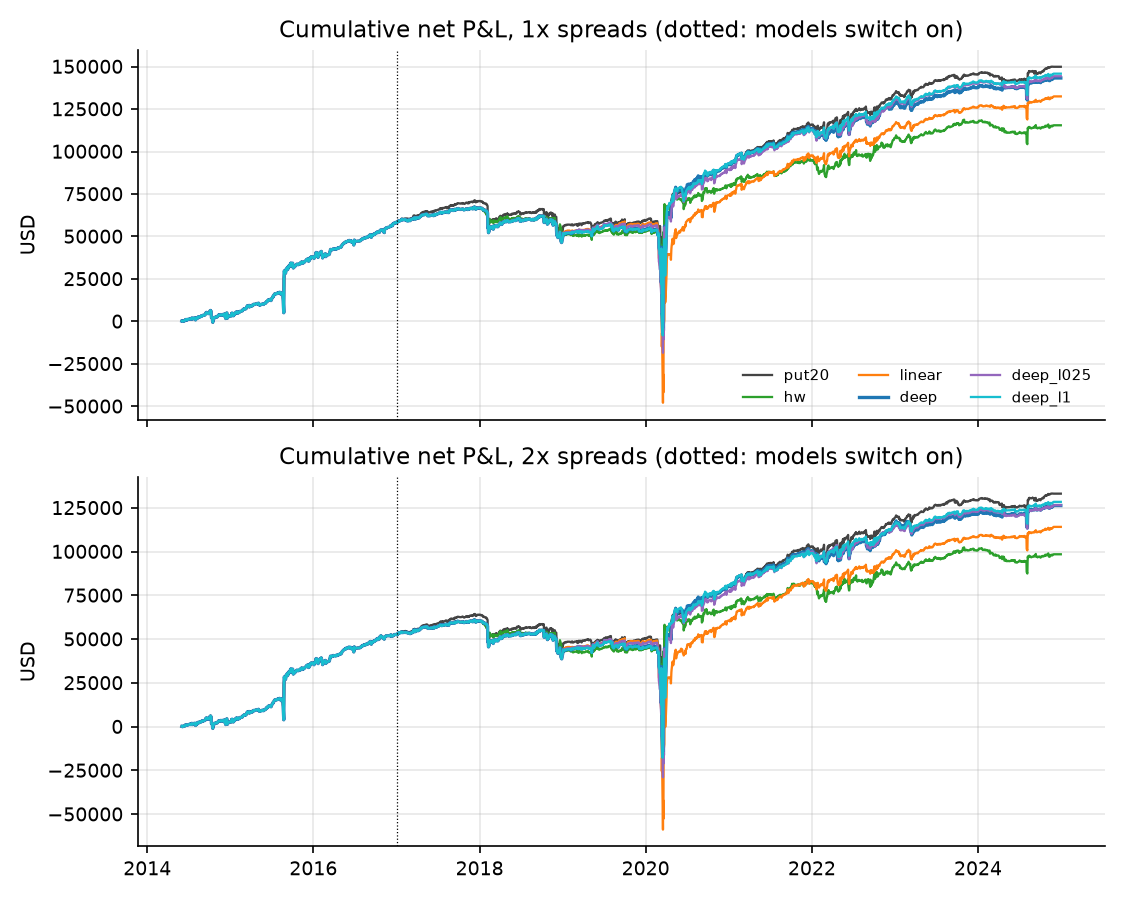
\includegraphics[width=0.92\linewidth]{figures/cum_pnl.png}\caption{Cumulative net P\&L, 1x (top) and 2x (bottom). Dotted line: models switch on, January 2017}\end{figure}

All lines are identical until January 2017. From then on \texttt{put20} stays at or near the top and ends highest at both spreads. The three \texttt{deep} variants follow it closely, a little below. \texttt{linear} falls furthest in March 2020 and never closes the gap. \texttt{hw} falls behind from the 2020 rebound onward and ends lowest.

\begin{figure}[H]\centering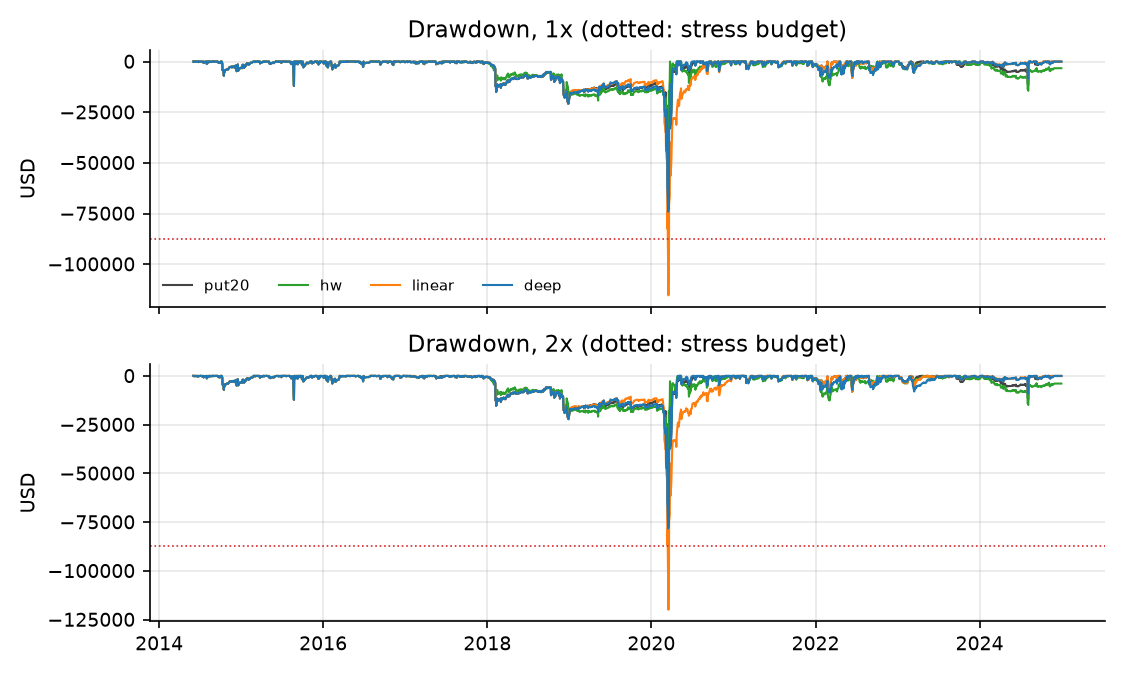
\includegraphics[width=0.92\linewidth]{figures/drawdown.png}\caption{Drawdown at 1x and 2x. Dotted line: the \$87,500 stress budget}\end{figure}

Every policy's worst drawdown is in March 2020. \texttt{put20}'s is \$48k at 1x; \texttt{deep} reaches \$74k, and \texttt{linear} goes through the stress budget to \$115k (1x) and \$120k (2x). \texttt{hw} has the smallest March 2020 drawdown (\$41k at 1x), but sits slightly deeper than the others in 2019, 2022 and 2024.

\begin{figure}[H]\centering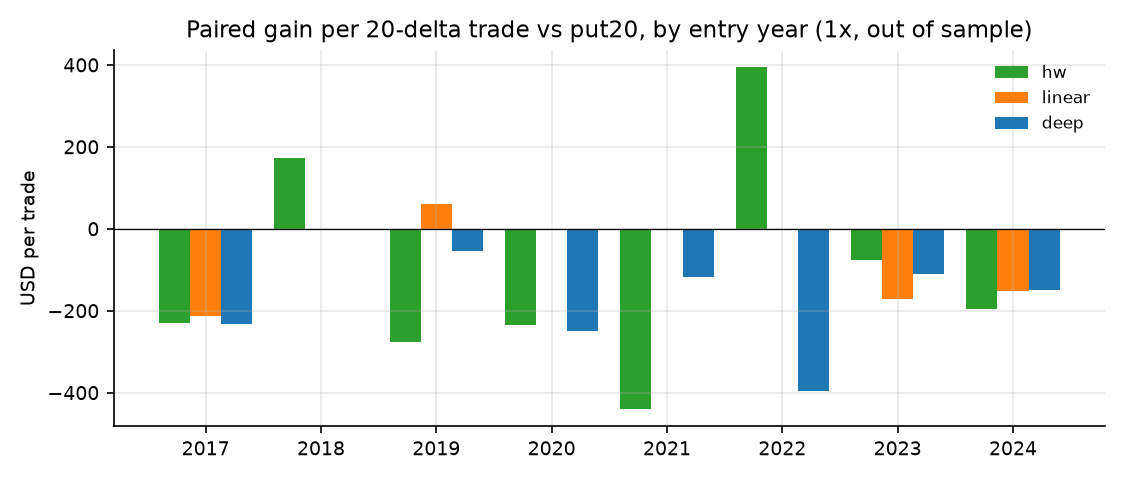
\includegraphics[width=0.92\linewidth]{figures/paired_by_year.png}\caption{Paired gain per 20-delta trade vs \texttt{put20}, by entry year (1x, out of sample)}\end{figure}

\texttt{deep} lost in every year except 2018, when early stopping chose pure delta and it matched \texttt{put20} exactly. Its worst year was 2022 ($-$\$395 per trade), then 2020 ($-$\$249) and 2017 ($-$\$231). \texttt{linear} gained only in 2019 (+\$61), and matched delta in 2018, 2021 and 2022. \texttt{hw} gained in 2018 (+\$173) and 2022 (+\$396), both falling years, and lost in the other six, most in 2021 ($-$\$440). The two sensitivities are not drawn: \texttt{deep\_\allowbreak{}l025} gained only in 2019 (+\$15) and matched delta in 2018 and 2021; \texttt{deep\_\allowbreak{}l1} matched delta in 2018 and 2022 and lost in every other year.

\begin{figure}[H]\centering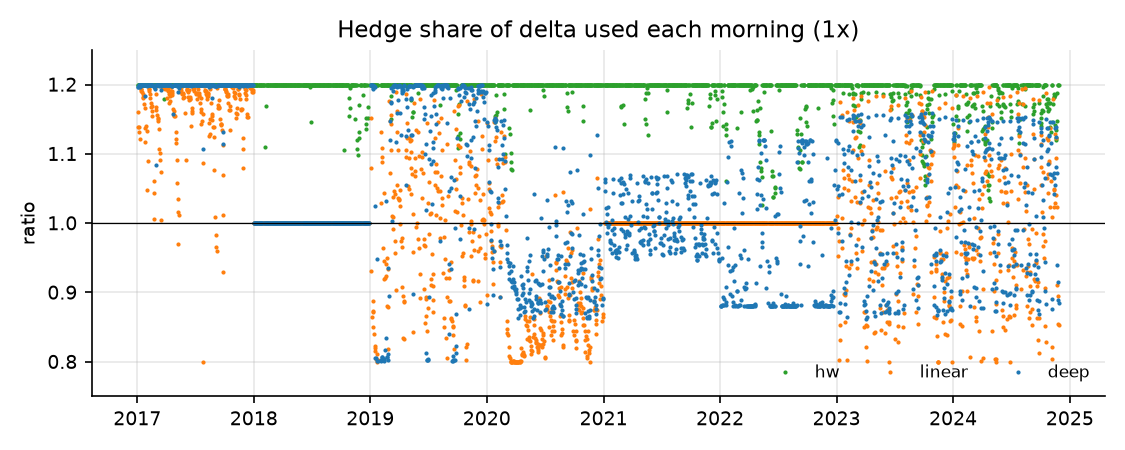
\includegraphics[width=0.92\linewidth]{figures/ratio.png}\caption{Hedge share of delta used each morning (1x)}\end{figure}

\texttt{hw} sits at the 1.2 cap almost every day from 2017 to 2022 and spreads between about 1.1 and 1.2 in 2023-2024, as its fitted coefficients shrink. \texttt{deep} hedges exactly 1.0 in 2018. Its 2020 model hedged mostly between 0.8 and 1.0 from the March crash to year end, and its 2022 model sat near 0.88 for much of the second half of 2022, the year of its largest paired loss. \texttt{linear} hedged 1.0 in 2021-2022 and sat at the 0.8 floor in March-April 2020.

\subsection{The net still leans the v1 way}

Mean hedge ratio by VIX level, 1x:

\begin{center}\small
\begin{tabular}{lccccccc}
\toprule
\textbf{Policy} & \textbf{VIX \ensuremath{\leq} 13} & \textbf{13-16} & \textbf{16-20} & \textbf{20-25} & \textbf{25-35} & \textbf{> 35} & \textbf{Mean} \\
\midrule
\texttt{deep} & 1.117 & 1.036 & 1.023 & 0.981 & 0.977 & 0.931 & 1.031 \\
\texttt{linear} & 1.076 & 1.001 & 1.008 & 0.986 & 0.951 & 0.842 & 1.006 \\
\texttt{hw} & 1.199 & 1.193 & 1.188 & 1.190 & 1.182 & 1.186 & 1.191 \\
\bottomrule
\end{tabular}
\end{center}

\texttt{deep} hedged about 1.12\ensuremath{\times} delta with VIX under 13 and about 0.93\ensuremath{\times} above 35: it hedges less as the market falls. This is a mild version of v1's buy-the-dip tilt (v1 went from about 129\% to 59\%), held in by the box. \texttt{linear} does the same, more strongly, at 0.84\ensuremath{\times} above VIX 35. \texttt{hw} is flat at the cap.

\subsection{Early stopping}

For each yearly model: the best epoch, the share of the 5 seeds whose best state was epoch 0 (pure delta), and the best validation objective (mean $-$ \ensuremath{\lambda} \ensuremath{\times} CVaR95, USD, on the last 20\% of the training window).

\begin{center}\footnotesize\setlength{\tabcolsep}{4pt}
\begin{tabular}{lcccccccc}
\toprule
 & \textbf{2017} & \textbf{2018} & \textbf{2019} & \textbf{2020} & \textbf{2021} & \textbf{2022} & \textbf{2023} & \textbf{2024} \\
\midrule
\texttt{deep}: best epoch & 320 & 0 & 200 & 40 & 20 & 380 & 40 & 40 \\
\quad seeds at delta & 0 & 1.0 & 0 & 0 & 0.2 & 0.4 & 0 & 0 \\
\quad best val.\ objective & \$821 & \$256 & $-$\$4,273 & $-$\$2,784 & $-$\$6,542 & \$588 & $-$\$2,041 & $-$\$1,923 \\
\quad paired gain (1x) & $-$\$231 & \$0 & $-$\$54 & $-$\$249 & $-$\$117 & $-$\$395 & $-$\$109 & $-$\$149 \\
\midrule
Variants stopped at delta & & all 6 & & & \texttt{l025}, \texttt{lin.} & \texttt{l1}, \texttt{lin.} & & \\
\bottomrule
\end{tabular}
\end{center}

Validation picked pure delta in 2018 for every variant (\texttt{deep}, both sensitivities, both seed sets, \texttt{linear}). That is the one year with no loss. In the other years it usually found a deviation that looked better on the last 20\% of the training window (about a year) and then lost the next year. The two \texttt{deep} models with a positive validation objective, 2017 and 2022, had two of its three largest out-of-sample losses. The validation window is too short and too noisy to pick a winner.

\subsection{Hull-White: ``hedge more'' is a risk dial}

The one real effect in the experiment is Hull-White's ``hedge more''. Hedging about 1.2\ensuremath{\times} delta (mean ratio 1.191) cut paired CVaR95 from \$8,590 to \$7,040 per trade at 1x ($-$18\%), and from \$8,945 to \$7,520 at 2x. In the engine it cut the 2017-2024 drawdown from \$48,435 to \$41,436 and ES 5\% from $-$\$2,705 to $-$\$2,532 at 1x. It cost \$34,438 of 2017-2024 P\&L at 1x (Sharpe 0.40 against 0.61). That is a trade of return for risk, not a source of return.

The walk-forward fit, by year:

\begin{center}\small
\begin{tabular}{lcccccccc}
\toprule
 & \textbf{2017} & \textbf{2018} & \textbf{2019} & \textbf{2020} & \textbf{2021} & \textbf{2022} & \textbf{2023} & \textbf{2024} \\
\midrule
a & $-$0.271 & $-$0.242 & $-$0.244 & $-$0.215 & $-$0.208 & $-$0.191 & $-$0.150 & $-$0.137 \\
b & $-$0.276 & $-$0.215 & $-$0.237 & $-$0.208 & $-$0.222 & $-$0.146 & $-$0.084 & $-$0.084 \\
c & $-$0.169 & $-$0.114 & $-$0.166 & $-$0.161 & $-$0.134 & $-$0.063 & $-$0.020 & $-$0.046 \\
R\textsuperscript{2} & 0.139 & 0.115 & 0.147 & 0.130 & 0.098 & 0.101 & 0.092 & 0.086 \\
Observations (k) & 132 & 174 & 232 & 290 & 366 & 446 & 536 & 608 \\
\bottomrule
\end{tabular}
\end{center}

a, b, c are the coefficients on (vega/\ensuremath{\sqrt{T}})(\ensuremath{\Delta}S/S) \ensuremath{\times} [1, \ensuremath{\delta}, \ensuremath{\delta^2}]; R\textsuperscript{2} is the share of the delta-hedge error's variance the fit explains. The coefficients shrink toward zero over time, which is why the cap stops binding in 2023-2024.

\subsection{Without February-April 2020}

Engine gain over \texttt{put20}, 2017-2024, 1x, split around 19 February-30 April 2020:

\begin{center}\small
\begin{tabular}{lrrr}
\toprule
\textbf{Policy} & \textbf{2017-2024} & \textbf{19 Feb-30 Apr 2020} & \textbf{Without that window} \\
\midrule
\texttt{deep} & $-$\$6,595 & +\$2,085 & $-$\$8,680 \\
\texttt{deep\_\allowbreak{}l025} & $-$\$5,566 & $-$\$3,013 & $-$\$2,553 \\
\texttt{deep\_\allowbreak{}l1} & $-$\$4,050 & +\$4,436 & $-$\$8,485 \\
\texttt{linear} & $-$\$17,439 & $-$\$25,221 & +\$7,782 \\
\texttt{hw} & $-$\$34,438 & +\$3,784 & $-$\$38,222 \\
\bottomrule
\end{tabular}
\end{center}

Unlike v1, the result does not hang on the crash: \texttt{deep} is behind both inside and outside it. Only \texttt{linear} is ahead outside the window, by \$7.8k, after losing \$25.2k inside it. Its paired test (one model, interval [$-$\$180, +\$54]) does not support that as a real effect.

The drawdown widened even though the hedge was bounded: \texttt{deep} reached \$74k against \$48k, at the same 16 March 2020 trough. It was about 7\% under-hedged into the crash (mean ratio 0.931 with VIX above 35) and its stops fired at different times.

\subsection{Simulator against engine}

The paired test runs in the training simulator. To check that it measures the right thing, the simulator was run on the 2014-2016 \texttt{put20} trades, which no model scores on:

\begin{center}\small
\begin{tabular}{cccccc}
\toprule
\textbf{Trades} & \textbf{Matched} & \textbf{Correlation} & \textbf{Median abs. gap} & \textbf{Simulator total} & \textbf{Engine total} \\
\midrule
48 & 48 & 0.92 & \$114 & \$59,004 & \$57,113 \\
\bottomrule
\end{tabular}
\end{center}

All 48 trades matched, per-trade P\&L correlates at 0.92, and the totals differ by \$1.9k. The simulator tracks the engine well, and the engine results agree with the paired test in direction for every policy.

\section{Caveats and disclosures}

\begin{itemize}

\item \textbf{The window was seen before.} v1 ran on 2017-2024, and this design (the 0.8-1.2 box, \ensuremath{\lambda}, the new inputs, early stopping) was chosen after v1's results. The risk tolerance is looser than v1's (ES within 1.25\ensuremath{\times} instead of 1.10\ensuremath{\times}; Sharpe up to 0.05 lower) because the PM asked for a strategy that may take slightly more risk if returns are proved. Reuse of the window biases toward a false pass, not a fail.

\item \textbf{The paired test runs in the simulator, not the engine,} on overlapping daily episodes, while the engine trades one put at a time. The pre-2017 reconciliation above is the check on this.

\item \textbf{Engine carry attribution.} When a new put takes over the previous put's leftover shares, \texttt{engine.\allowbreak{}carry()} books them at the decision-view spot, while hedge trades fill at the fill-view spot. This shifts a few hundred to a couple of thousand dollars between trades and can move a stop by a day. Book-level equity is unaffected. It hits every book, \texttt{put20} included, and is not fixed here.

\item \textbf{Training gaps.} Stress sizing still assumes a full hedge, so a 0.8\ensuremath{\times} hedge carries more risk than the sizing allows for. The model switches on 1 January even mid-trade.

\item \textbf{Linear is one model.} Its 5 seeds train identically, so its result has no ensemble averaging.

\end{itemize}

\section{Conclusion and next steps}

Failed, per the pre-registered bar. Archive this card. Two attempts (16 trials) agree that for \texttt{put20}, a learned daily hedge ratio does not add return over plain delta hedging. Within \ensuremath{\pm}20\% it costs about \$100-160 per trade out of sample; unbounded (v1), it turned into a crash bet.

\begin{enumerate}

\item \textbf{Stop pursuing the hedge as a return source} for this book.

\item \textbf{If the desk wants a smaller tail,} write a card for a fixed over-hedge (for example 1.1-1.2\ensuremath{\times} delta, or Hull-White) as an explicit trade of return for risk, judged on drawdown and CVaR per dollar of P\&L given up.

\item \textbf{Fix the engine's carry attribution} (\texttt{engine.\allowbreak{}carry()} should price at the fill spot) on its own branch. It changes every registered result, so the PM should decide.

\item \textbf{Look elsewhere for return:} exit rules (stop and profit-take), strike and sizing, where the earlier experiments show the path effects sit.

\end{enumerate}

\end{document}
